\documentclass[tikz,border=4pt]{standalone}
\usepackage{amsmath}
\begin{document}
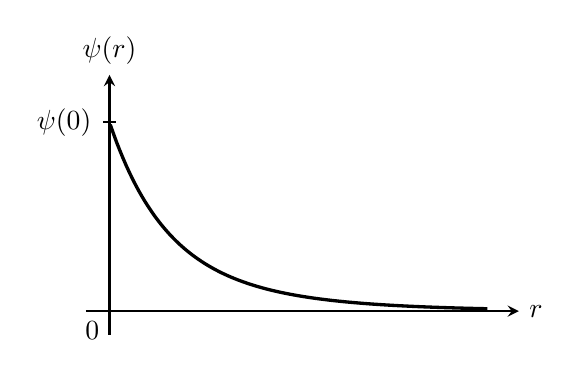
\begin{tikzpicture}[>=stealth, thick, scale=1.0]
  % Axes
  \draw[->] (-0.3, 0) -- (5.2, 0) node[right] {$r$};
  \draw[->] (0, -0.3) -- (0, 3.0) node[above] {$\psi(r)$};
  \node[below left] at (0, 0) {$0$};

  % Plot (exp(-0.5*x) - exp(-2.0*x)) / x, scaled by 1.6 (value at 0 is 1.5 -> 2.4)
  \draw[very thick, domain=0.01:4.8, samples=120]
    plot (\x, {1.6 * (exp(-0.5*\x) - exp(-2.0*\x)) / \x});

  % Value at r=0
  \draw (-0.08, 2.4) -- (0.08, 2.4);
  \node[left] at (-0.1, 2.4) {$\psi(0)$};
\end{tikzpicture}
\end{document}
